\documentclass{beamer}


\input{./estruturasDeDados.tex}

\newcommand{\tituloaula}{Introdução às \'{A}rvores}
\usepackage{framed}
% Titulo
\title[\sc{Estruturas de Informação I}]{Estruturas de Informação I}
\subtitle{\tituloaula}
 
\usetikzlibrary{shapes,arrows,calc}
\newcommand{\data}{data \nodepart{second} \phantom{null}}

\tikzstyle{ptr}  = [draw, -latex']
\tikzstyle{head} = [rectangle, draw, text height=3mm, text width=3mm, text centered, node distance=3cm, inner sep=0pt]
\tikzstyle{data} = [rectangle split, rectangle split parts=2, draw, text centered, minimum height=3em]

\tikzset{
  htree leaves/.initial=2,
  sibling angle/.initial=20,
  htree level/.initial={}
}
\makeatletter

\def\htree@growth{%
  \pgftransformrotate{%
    (\pgfkeysvalueof{/tikz/sibling angle})*(-.5-.5*\tikznumberofchildren
      +\tikznumberofcurrentchild)}%
  \pgftransformxshift{\the\tikzleveldistance}%
  \pgfkeysvalueof{/tikz/htree level}%
}
\tikzstyle{htree}=[
  growth function=\htree@growth,
  sibling angle=180,
  htree level={
    \tikzleveldistance=.707\tikzleveldistance
    \pgfsetlinewidth{.707*\the\pgflinewidth}
  }
]

\tikzstyle{btree}=[
  growth function=\htree@growth,
  sibling angle=60,
  htree level={
    \tikzleveldistance=.55\tikzleveldistance
    \pgfsetlinewidth{.707*\the\pgflinewidth}
  }
]

\long\def\ge@addto@macro#1#2{%
  \begingroup
  \toks@\expandafter\expandafter\expandafter{\expandafter#1#2}%
  \xdef#1{\the\toks@}%
  \endgroup}

\newcommand{\htree}[2][]{%
  \def\htree@start{\noexpand\coordinate}
  \def\htree@end{}
  \foreach \l in {0,...,#2} {
    \g@addto@macro\htree@start{child foreach \noexpand\x in {1,2} {\iffalse}\fi}
    \g@addto@macro\htree@end{\iffalse{\fi}}
    \global\let\htree@start\htree@start
    \global\let\htree@end\htree@end
  }
  \edef\htree@cmd{\htree@start\htree@end;}
  \begin{scope}[htree,#1]
  \htree@cmd
  \end{scope}
}

\makeatother
\begin{document}

\begin{frame}
  \titlepage 
\end{frame}

\begin{frame}
	\frametitle{Resumo}
	\tableofcontents
\end{frame}

\section{EI14 -  \tituloaula}
\begin{frame}
\frametitle{Estruturas de Dados Lineares}
Array: \includegraphics[scale=0.2]{imagens/img18}
	

Lista Encadeada:
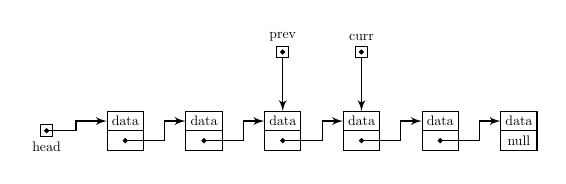
\begin{tikzpicture}[node distance=2cm, auto, scale=0.5, transform shape]

    \node[head, label=below:head] (head) {};
    \node[data, right of=head]    (A) {\data};
    \node[data, right of=A]       (B) {\data};
    \node[data, right of=B]       (C) {\data};
    \node[above of=C,head,node distance=2cm,label=above:prev]   (prev){};
    \node[data, right of=C]       (D) {\data};
    \node[above of=D,head,node distance=2cm,label=above:curr]   (curr){};
    \node[data, right of=D]       (E) {\data};
    \node[data, right of=E]       (last) {data \nodepart{second} null};

    \draw[fill] (head.center)   circle (0.05);
    \draw[fill] (prev.center)   circle (0.05);
    \draw[fill] (curr.center)   circle (0.05);

    \path[ptr]  (head.center) --++(right:7.5mm)  |- (A.text west);
    \draw[fill] ($(A.south)!0.5!(A.text split)$) circle (0.05);
    \draw[ptr]  ($(A.south)!0.5!(A.text split)$) --++(right:10mm) |- (B.text west);
    \draw[fill] ($(B.south)!0.5!(B.text split)$) circle (0.05);
    \draw[ptr]  ($(B.south)!0.5!(B.text split)$) --++(right:10mm) |- (C.text west);
    \path[ptr] (prev) -- (C);
    \draw[fill] ($(C.south)!0.5!(C.text split)$) circle (0.05);
    \draw[ptr]  ($(C.south)!0.5!(C.text split)$) --++(right:10mm) |- (D.text west);
    \path[ptr] (curr) -- (D);
    \draw[fill] ($(D.south)!0.5!(D.text split)$) circle (0.05);
    \draw[ptr]  ($(D.south)!0.5!(D.text split)$) --++(right:10mm) |- (E.text west);
    \draw[fill] ($(E.south)!0.5!(E.text split)$) circle (0.05);
    \draw[ptr]  ($(E.south)!0.5!(E.text split)$) --++(right:10mm) |- (last.text west);

\end{tikzpicture}

Pilha

Skiplist

Fila

\end{frame}


\begin{frame}
\frametitle{Quais fatores são importantes para escolher uma estrutura de dados?}\pause

\begin{itemize}
\item O que vai ser armazenado?\pause
\item Qual o custo das operações?\pause
\item Qual o uso de memória?\pause
\item A implementação é fácil?
\end{itemize}
\end{frame}

\begin{frame}
\frametitle{O que é uma árvore?}
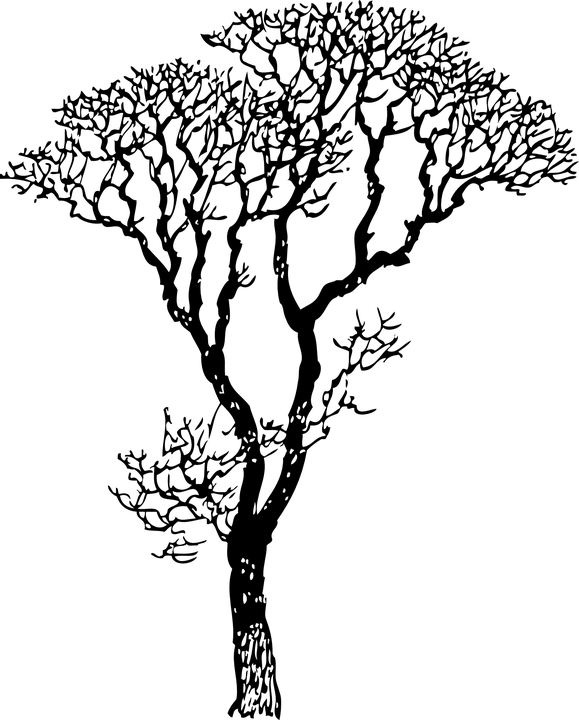
\includegraphics[scale=0.3]{imagens/arvore}

\end{frame}



\begin{frame}
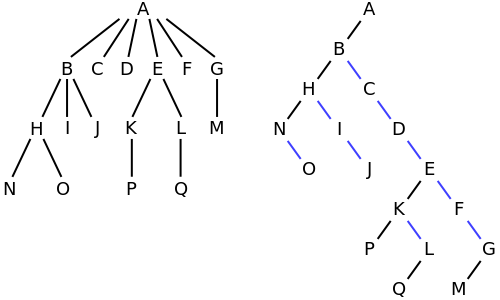
\includegraphics[scale=0.5]{imagens/Nary_to_binary}
\frametitle{Definição Formal de Árvore}
Formalmente, definimos uma \textbf{árvore T} como um conjunto de nós de armazenamento, de tal modo que os nós possuem uma relação \textbf{pai-filho} que satisfaz às seguintes propriedades:
\begin{itemize}
\item Se \textbf{T} não é vazia, existe um nó especial, chamado \textbf{raiz de T}, que não possui nó pai.
\item Cada nó \textbf{v} de \textbf{T} diferente da raiz possui um único parente \textbf{w}. Cada nó com pai \textbf{w} é um \textbf{filho de w}.
\end{itemize}

\end{frame}

\begin{frame}
\frametitle{Relações entre nós}
Dois nós que são filhos do mesmo pai são \textbf{irmãos}. Um nó \textbf{v} é \textbf{externo} se v não possui filhos. Um nó \textbf{v} é \textbf{interno} se ele possui um ou mais filhos. Nós externos são conhecidos também como \textbf{folhas}.


\end{frame}

\begin{frame}
\frametitle{Ascendentes e Descendentes}
Um nó \textbf{u} é um \textbf{ascendente} de um nó v se \textbf{u é pai de v} ou \textbf{u} é um \textbf{ascendente do pai de v}. Do mesmo modo, dizemos que um nó \textbf{v} é um \textbf{descendente} de um nó u se \textbf{u é um ascendente de v}.
.
\end{frame}

\begin{frame}
\frametitle{Arestas e percursos}
Uma \textbf{aresta} da árvore T é um par de nós \textbf{(u, v)} tal que \textbf{u} é pai de \textbf{v} ou vice-versa. Um \textbf{caminho} de T é uma sequência de nós tal que quaisquer dois nós consecutivos na sequência formam uma aresta.
\end{frame}

\begin{frame}
\frametitle{Árvores Ordenadas}
Uma árvore é ordenada se existe uma ordem significativa entre os filhos de cada nó, isto é, identificamos os filhos de um nó como sendo primeiro, segundo, terceiro e assim por diante. Tal ordem é normalmente visualizada arranjando os irmãos da esquerda para direita, de acordo com sua ordem.
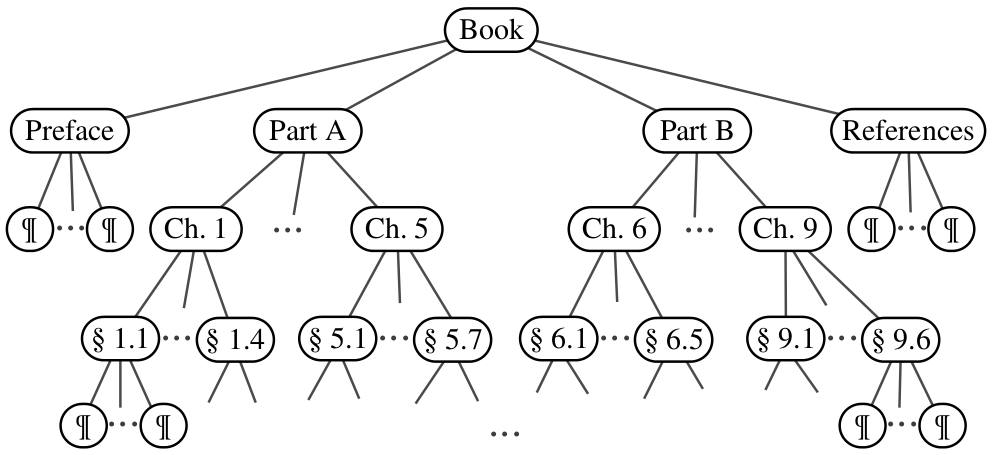
\includegraphics[scale=0.35]{imagens/arvoredelivros}
\end{frame}







\begin{frame}
\frametitle{Profundidade}
\textbf{Nível} ou \textbf{profundidade} de um nó de uma árvore \textbf{T} é o comprimento do caminho entre a raiz e o nó.

A \textbf{raiz} está no nível \textbf{zero} e seus filhos estão no nível 1.

Uma definição mais formal seria:
\begin{itemize}
\item Se \textbf{p} é a \textbf{raiz}, então sua profundidade é \textbf{0}.
\item Caso contrário, a \textbf{profundidade} de \textbf{p} é um mais a \textbf{profundidade} do pai de \textbf{p}.
\end{itemize}
\end{frame}

\begin{frame}
\frametitle{Altura de um nó}

A altura da posição p na árvore T também pode ser definida recursivamente:
\begin{itemize}
\item Se \textbf{p} é uma \textbf{folha}, então a \textbf{altura} de \textbf{p} é \textbf{0}.
\item Caso contrário, a \textbf{altura de p} é um mais o \textbf{máximo} da altura dos filhos de \textbf{p}.
\end{itemize}

Proposição:

A \textbf{altura} de uma árvore não vazia \textbf{T} é igual ao \textbf{máximo da profundidade} das suas \textbf{folhas}.
\end{frame}



\section{6.1 Árvore Binária}
\begin{frame}
\frametitle{Árvore Binária}

Uma \textbf{árvore binária} é uma árvore ordenada com as seguintes propriedades:
\begin{enumerate}
\item Cada nó possui no máximo dois filhos.
\item Cada nó filho é marcado como sendo filho \textbf{esquerdo} ou filho \textbf{direito}.
\item O filho esquerdo precede o filho direito na ordem dos filhos de um nó.
\end{enumerate}
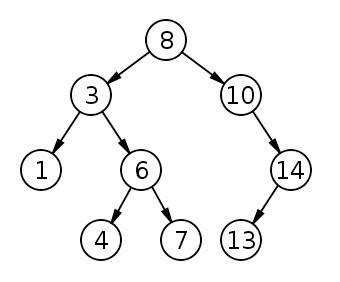
\includegraphics[scale=0.5]{imagens/ArvoreBinaria1}
\end{frame}

\begin{frame}
\frametitle{Exemplo}

Uma expressão aritmética pode ser representada por uma árvore binária cujas folhas são associadas com variáveis ou constantes, e cujos nós internos são associados com os operadores  + , - , x , e / . Cada nó em tal árvore tem um valor associado
\begin{itemize}
\item Se um nó é uma folha, então seu valor é aquele da variável ou constante.
\item Se o nó é interno, então seu valor é definido pela aplicação da operação para os valores de seus filhos.
\end{itemize}
\end{frame}

\begin{frame}
\frametitle{Expressão aritmética}

Esta árvore representa a expressão ((((3 + 1) x 3)/((9 - 5) + 2)) - ((3 x (7 - 4)) + 6)). O valor associado com o nó interno  ``/'' é 2.

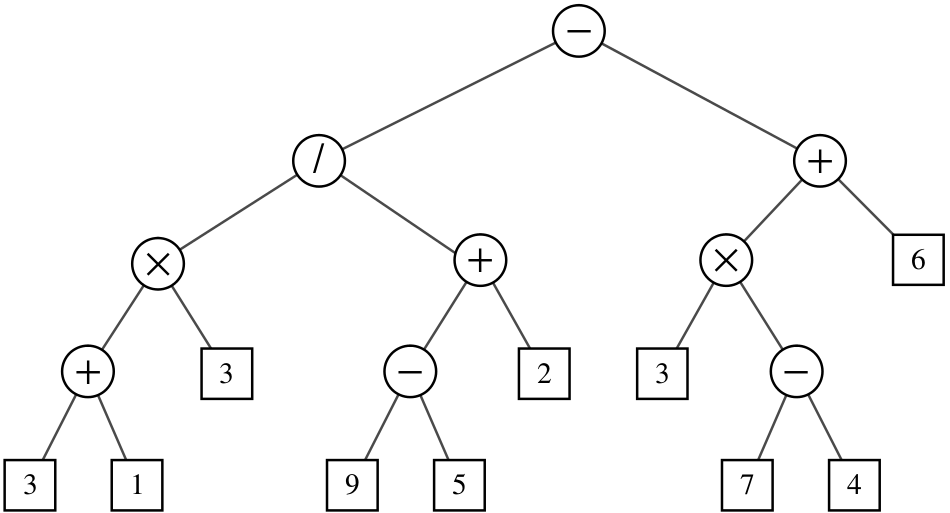
\includegraphics[scale=0.4]{imagens/arvorebinaria}
\end{frame}



\begin{frame}
\frametitle{Propriedades das Árvores Binárias}
Árvores binárias possuem algumas propriedades interessantes devido ao relacionamento entre suas alturas e o número de nós. Indicamos o conjunto de todos os nós de uma mesma profundidade d de uma árvore T como o nível d de T. Na árvore binária o nível 0 tem no máximo 1 nó, o nível 1 no máximo 2 nós, o nível 2 no máximo 4 nós e assim por diante. Generalizando, o nível d possui no máximo $2^d$ nós.
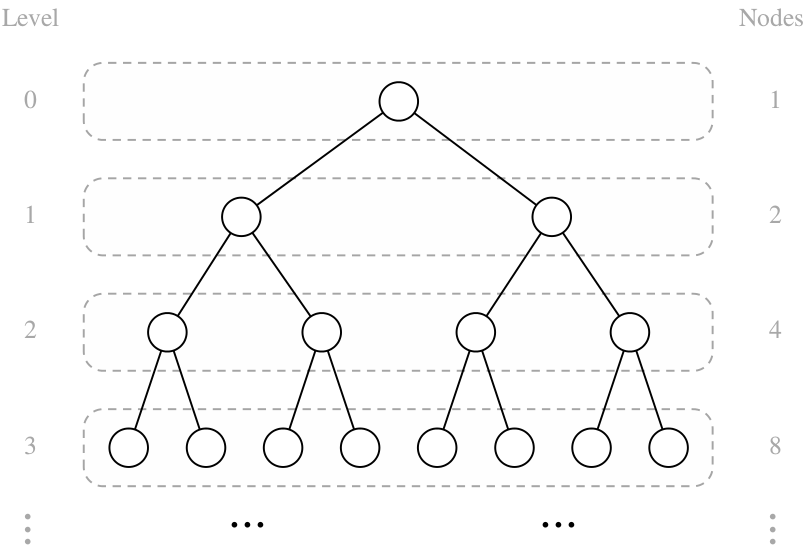
\includegraphics[scale=0.3]{imagens/arvorebinaria1}
\end{frame}

\begin{frame}
\frametitle{Proposição}
Seja T uma árvore binária não vazia, e sejam $n$, $n_E$, $n_I$ e $h$ indicarem o número de nós, o número de nós externos, o número de nós internos e a altura de T, respectivamente. Então T possui as seguintes propriedades:
\begin{enumerate}
\item $h + 1 \leq n \leq 2^{h+1} - 1$
\item $1 \leq n_E \leq 2^h$
\item $h \leq n_I \leq 2^h - 1$
\item $log(n + 1) - 1 \leq h \leq n - 1$
\end{enumerate}

\end{frame}

\begin{frame}
\frametitle{Árvore estritamente binária}
Uma árvore ``estritamente binária'' é uma árvore na qual todo nó tem zero ou duas folhas. Esta árvore possui as seguintes propriedades adiconais:

\begin{enumerate}
\item $2h + 1 \leq n \leq 2^{h+1}  - 1$
\item $h + 1 \leq  n_E \leq  2^h$
\item $h \leq  n_I \leq  2^h - 1$
\item $log(n + 1) - 1 \leq  h \leq  (n - 1)/2$
\end{enumerate}

\end{frame}

\begin{frame}
\frametitle{Árvore binária implementada como Lista Encadeada}

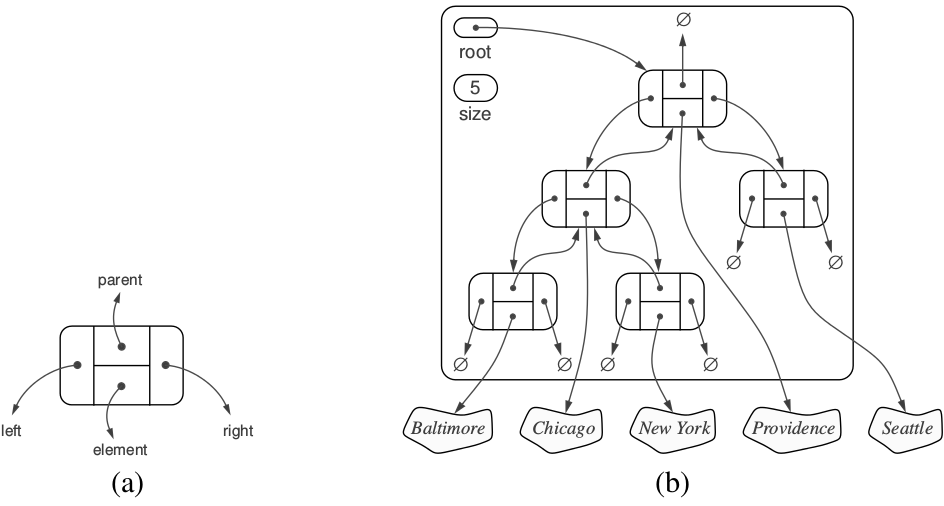
\includegraphics[scale=0.48]{imagens/arvorebinaria2}

\end{frame}

\begin{frame}
\frametitle{$initialize()$}

A própria árvore binária pode ser representada por uma
referência ao seu nó raiz, $r$:
%importing \codeimport{ods/ArvoreBinaria.r}: 
\begin{oframed}
\begin{flushleft}
\hspace*{1em} \ensuremath{\mathrm{initialize}()}\\
\hspace*{1em} \hspace*{1em} \ensuremath{\ensuremath{\mathit{raiz}} \gets  \ensuremath{nil}}\\
\end{flushleft}
\end{oframed}
\end{frame}

\begin{frame}
\frametitle{$profundidade()$}
Podemos calcular a profundidade de um nó, \ensuremath{\ensuremath{\ensuremath{\mathit{u}}}}, em uma árvore binária contando
o número de passos no caminho de \ensuremath{\ensuremath{\ensuremath{\mathit{u}}}} até a raiz:
%importing \codeimport{ods/ArvoreBinaria.profundidade(u)}: 
\begin{oframed}
\begin{flushleft}
\hspace*{1em} \ensuremath{\mathrm{profundidade}(\ensuremath{\mathit{u}})}\\
\hspace*{1em} \hspace*{1em} \ensuremath{\ensuremath{\mathit{profund}} \gets  \ensuremath{0}}\\
\hspace*{1em} \hspace*{1em} {\color{black} \textbf{while}} \ensuremath{(\ensuremath{\mathit{u}} \ne \ensuremath{\mathit{raiz}})} {\color{black} \textbf{do}} \\
\hspace*{1em} \hspace*{1em} \hspace*{1em} \ensuremath{\ensuremath{\mathit{u}} \gets  \ensuremath{\ensuremath{\mathit{u}}.pai}}\\
\hspace*{1em} \hspace*{1em} \hspace*{1em} \ensuremath{\ensuremath{\mathit{profund}} \gets  \ensuremath{\ensuremath{\mathit{profund}} + 1}}\\
\hspace*{1em} \hspace*{1em} {\color{black} \textbf{return}} \ensuremath{\ensuremath{\mathit{profund}}}\\
\end{flushleft}
\end{oframed}
\end{frame}

\begin{frame}
\frametitle{Recursão}
Usar algoritmos recursivos torna muito fácil o cálculo envolvendo árvores binárias. Por exemplo, para calcular o tamanho (número de nós) de uma
árvore binária com raízes no nó \ensuremath{\ensuremath{\ensuremath{\mathit{u}}}}, recursivamente calculamos o tamanho
das duas subárvores com raiz nos filhos de \ensuremath{\ensuremath{\ensuremath{\mathit{u}}}}, somamos os tamanhos e adicionamos um:

%importing \codeimport{ods/ArvoreBinaria.tamanho(u)}: 
\begin{oframed}
\begin{flushleft}
\hspace*{1em} \ensuremath{\mathrm{tamanho}(\ensuremath{\mathit{u}})}\\
\hspace*{1em} \hspace*{1em} {\color{black} \textbf{if}} \ensuremath{\ensuremath{\mathit{u}} = nil} {\color{black} \textbf{then}}  {\color{black} \textbf{return}} \ensuremath{0}\\
\hspace*{1em} \hspace*{1em} {\color{black} \textbf{return}} \ensuremath{1 + \mathrm{tamanho}(\ensuremath{\mathit{u}}.\ensuremath{\mathit{esquerdo}}) + \mathrm{tamanho}(\ensuremath{\mathit{u}}.\ensuremath{\mathit{direito}})}\\
\end{flushleft}
\end{oframed}
\end{frame}

\begin{frame}
\frametitle{altura}
Para calcular a altura de um nó \ensuremath{\ensuremath{\ensuremath{\mathit{u}}}}, podemos calcular a altura das duas subárvores de \ensuremath{\ensuremath{\ensuremath{\mathit{u}}}}, pegar o valor máximo e adicionar 1:

%importing \codeimport{ods/ArvoreBinaria.altura(u)}: 
\begin{oframed}
\begin{flushleft}
\hspace*{1em} \ensuremath{\mathrm{altura}(\ensuremath{\mathit{u}})}\\
\hspace*{1em} \hspace*{1em} {\color{black} \textbf{if}} \ensuremath{\ensuremath{\mathit{u}} = nil} {\color{black} \textbf{then}}  {\color{black} \textbf{return}} \ensuremath{0}\\
\hspace*{1em} \hspace*{1em} {\color{black} \textbf{return}} \ensuremath{1 + \mathrm{max}(\mathrm{altura}(\ensuremath{\mathit{u}}.\ensuremath{\mathit{esquerdo}}), \mathrm{altura}(\ensuremath{\mathit{u}}.\ensuremath{\mathit{direito}})})\\
\end{flushleft}
\end{oframed}
\end{frame}

\begin{frame}
\frametitle{Percurso em árvores binárias}
\begin{oframed}
\begin{flushleft}
\hspace*{1em} \ensuremath{\mathrm{percurso}(\ensuremath{\mathit{u}})}\\
\hspace*{1em} \hspace*{1em} {\color{black} \textbf{if}} \ensuremath{\ensuremath{\mathit{u}} =nil} {\color{black} \textbf{then}}  {\color{black} \textbf{return}}\\
\hspace*{1em} \hspace*{1em} \ensuremath{\mathrm{percurso}(\ensuremath{\mathit{u}}.\ensuremath{\mathit{esquerdo}})}\\
\hspace*{1em} \hspace*{1em} \ensuremath{\mathrm{percurso}(\ensuremath{\mathit{u}}.\ensuremath{\mathit{direito}})}\\
\end{flushleft}
\end{oframed}
\end{frame}

\begin{frame}
\frametitle{Problema da recursão}
A profundidade máxima da recursão é dada pela
profundidade máxima do nó na árvore binária, i.e., a altura da árvore.
Se a altura da árvore é muito grande, então essa recursão pode muito bem utilizar mais espaço da pilha do que esteja disponível, causando um fechamento do programa.
\end{frame}

\begin{frame}
\frametitle{Percurso sem recursão}
Para percorrer uma árvore binária sem utilizar a recursão, você pode usar um algoritmo que
se baseie de onde ele vem para saber para onde vai.  Se chegamos ao nó \ensuremath{\ensuremath{\ensuremath{\mathit{u}}}} a partir de \ensuremath{\ensuremath{\ensuremath{\mathit{u}}.\ensuremath{\mathit{pai}}}},
então a próxima coisa a ser feita é visitar \ensuremath{\ensuremath{\ensuremath{\mathit{u}}.\ensuremath{\mathit{esquerdo}}}}.  Se chegamos a \ensuremath{\ensuremath{\ensuremath{\mathit{u}}}}
por \ensuremath{\ensuremath{\ensuremath{\mathit{u}}.\ensuremath{\mathit{esquerdo}}}}, então a próxima coisa a ser feita é visitar \ensuremath{\ensuremath{\ensuremath{\mathit{u}}.\ensuremath{\mathit{direito}}}}.  Se chegamos 
em \ensuremath{\ensuremath{\ensuremath{\mathit{u}}}} por \ensuremath{\ensuremath{\ensuremath{\mathit{u}}.\ensuremath{\mathit{direito}}}}, então terminamos de visitar a subárvore de \ensuremath{\ensuremath{\ensuremath{\mathit{u}}}},
e retornamos para \ensuremath{\ensuremath{\ensuremath{\mathit{u}}.\ensuremath{\mathit{pai}}}}.
\begin{figure}
  \begin{center}
    \begin{tabular}{cc}
      \includegraphics[scale=0.90909]{imagens/bintree-traverse-2}
      \includegraphics[scale=0.90909]{imagens/bintree-3}
    \end{tabular}
  \end{center}
\end{figure}
\end{frame}

\begin{frame}[shrink]
\frametitle{$percurso2()$}
\begin{oframed}
\begin{flushleft}
\hspace*{1em} \ensuremath{\mathrm{percurso2}()}\\
\hspace*{1em} \hspace*{1em} \ensuremath{\ensuremath{\mathit{u}} \gets  \ensuremath{raiz}}\\
\hspace*{1em} \hspace*{1em} \ensuremath{\ensuremath{\mathit{ant}} \gets  \ensuremath{nil}}\\
\hspace*{1em} \hspace*{1em} {\color{black} \textbf{while}} \ensuremath{\ensuremath{\mathit{u}} \ne nil} {\color{black} \textbf{do}} \\
\hspace*{1em} \hspace*{1em} \hspace*{1em} {\color{black} \textbf{if}} \ensuremath{\ensuremath{\mathit{ant}} =\ensuremath{\mathit{u}}.pai} {\color{black} \textbf{then}} \\
\hspace*{1em} \hspace*{1em} \hspace*{1em} \hspace*{1em} {\color{black} \textbf{if}} \ensuremath{\ensuremath{\mathit{u}}.\ensuremath{\mathit{esquerdo}} \ne nil} {\color{black} \textbf{then}}  \ensuremath{\ensuremath{\mathit{prox}} \gets  \ensuremath{\ensuremath{\mathit{u}}.esquerdo}}\\
\hspace*{1em} \hspace*{1em} \hspace*{1em} \hspace*{1em} {\color{black} \textbf{else}} {\color{black} \textbf{if}} \ensuremath{\ensuremath{\mathit{u}}.\ensuremath{\mathit{direito}} \ne nil} \ensuremath{\ensuremath{\mathit{prox}} \gets  \ensuremath{\ensuremath{\mathit{u}}.direito}}\\
\hspace*{1em} \hspace*{1em} \hspace*{1em} \hspace*{1em} {\color{black} \textbf{else}}  \ensuremath{\ensuremath{\mathit{prox}} \gets  \ensuremath{\ensuremath{\mathit{u}}.pai}}\\
\hspace*{1em} \hspace*{1em} \hspace*{1em} {\color{black} \textbf{else}} {\color{black} \textbf{if}} \ensuremath{\ensuremath{\mathit{ant}} = \ensuremath{\mathit{u}}.\ensuremath{\mathit{esquerdo}}}\\
\hspace*{1em} \hspace*{1em} \hspace*{1em} \hspace*{1em} {\color{black} \textbf{if}} \ensuremath{\ensuremath{\mathit{u}}.\ensuremath{\mathit{direito}} \ne nil} {\color{black} \textbf{then}}  \ensuremath{\ensuremath{\mathit{prox}} \gets  \ensuremath{\ensuremath{\mathit{u}}.direito}}\\
\hspace*{1em} \hspace*{1em} \hspace*{1em} \hspace*{1em} {\color{black} \textbf{else}}  \ensuremath{\ensuremath{\mathit{prox}} \gets  \ensuremath{\ensuremath{\mathit{u}}.pai}}\\
\hspace*{1em} \hspace*{1em} \hspace*{1em} {\color{black} \textbf{else}} \\
\hspace*{1em} \hspace*{1em} \hspace*{1em} \hspace*{1em} \ensuremath{\ensuremath{\mathit{prox}} \gets  \ensuremath{\ensuremath{\mathit{u}}.pai}}\\
\hspace*{1em} \hspace*{1em} \hspace*{1em} \ensuremath{\ensuremath{\mathit{ant}} \gets  \ensuremath{u}}\\
\hspace*{1em} \hspace*{1em} \hspace*{1em} \ensuremath{\ensuremath{\mathit{u}} \gets  \ensuremath{prox}}\\
\end{flushleft}
\end{oframed}
\end{frame}

\begin{frame}[shrink]
\frametitle{Tamanho sem recursão}
\begin{oframed}
\begin{flushleft}
\hspace*{1em} \ensuremath{\mathrm{tamanho2}()}\\
\hspace*{1em} \hspace*{1em} \ensuremath{\ensuremath{\mathit{u}} \gets  \ensuremath{raiz}}\\
\hspace*{1em} \hspace*{1em} \ensuremath{\ensuremath{\mathit{ant}} \gets  \ensuremath{nil}}\\
\hspace*{1em} \hspace*{1em} \ensuremath{\ensuremath{\mathit{n}} \gets  \ensuremath{0}}\\
\hspace*{1em} \hspace*{1em} {\color{black} \textbf{while}} \ensuremath{\ensuremath{\mathit{u}} \ne nil} {\color{black} \textbf{do}} \\
\hspace*{1em} \hspace*{1em} \hspace*{1em} {\color{black} \textbf{if}} \ensuremath{\ensuremath{\mathit{ant}} = \ensuremath{\mathit{u}}.pai} {\color{black} \textbf{then}} \\
\hspace*{1em} \hspace*{1em} \hspace*{1em} \hspace*{1em} \ensuremath{\ensuremath{\mathit{n}} \gets  \ensuremath{\ensuremath{\mathit{n}} + 1}}\\
\hspace*{1em} \hspace*{1em} \hspace*{1em} \hspace*{1em} {\color{black} \textbf{if}} \ensuremath{\ensuremath{\mathit{u}}.\ensuremath{\mathit{esquerdo}} \ne nil} {\color{black} \textbf{then}}  \ensuremath{\ensuremath{\mathit{prox}} \gets  \ensuremath{\ensuremath{\mathit{u}}.esquerdo}}\\
\hspace*{1em} \hspace*{1em} \hspace*{1em} \hspace*{1em} {\color{black} \textbf{else}} {\color{black} \textbf{if}} \ensuremath{\ensuremath{\mathit{u}}.\ensuremath{\mathit{direito}} \ne nil} \ensuremath{\ensuremath{\mathit{prox}} \gets  \ensuremath{\ensuremath{\mathit{u}}.direito}}\\
\hspace*{1em} \hspace*{1em} \hspace*{1em} \hspace*{1em} {\color{black} \textbf{else}}  \ensuremath{\ensuremath{\mathit{prox}} \gets  \ensuremath{\ensuremath{\mathit{u}}.pai}}\\
\hspace*{1em} \hspace*{1em} \hspace*{1em} {\color{black} \textbf{else}} {\color{black} \textbf{if}} \ensuremath{\ensuremath{\mathit{ant}} = \ensuremath{\mathit{u}}.\ensuremath{\mathit{esquerdo}}}\\
\hspace*{1em} \hspace*{1em} \hspace*{1em} \hspace*{1em} {\color{black} \textbf{if}} \ensuremath{\ensuremath{\mathit{u}}.\ensuremath{\mathit{direito}} \ne nil} {\color{black} \textbf{then}}  \ensuremath{\ensuremath{\mathit{prox}} \gets  \ensuremath{\ensuremath{\mathit{u}}.direito}}\\
\hspace*{1em} \hspace*{1em} \hspace*{1em} \hspace*{1em} {\color{black} \textbf{else}}  \ensuremath{\ensuremath{\mathit{prox}} \gets  \ensuremath{\ensuremath{\mathit{u}}.pai}}\\
\hspace*{1em} \hspace*{1em} \hspace*{1em} {\color{black} \textbf{else}} \\
\hspace*{1em} \hspace*{1em} \hspace*{1em} \hspace*{1em} \ensuremath{\ensuremath{\mathit{prox}} \gets  \ensuremath{\ensuremath{\mathit{u}}.pai}}\\
\hspace*{1em} \hspace*{1em} \hspace*{1em} \ensuremath{\ensuremath{\mathit{ant}} \gets  \ensuremath{u}}\\
\hspace*{1em} \hspace*{1em} \hspace*{1em} \ensuremath{\ensuremath{\mathit{u}} \gets  \ensuremath{prox}}\\
\hspace*{1em} \hspace*{1em} {\color{black} \textbf{return}} \ensuremath{n} \\
\end{flushleft}
\end{oframed}
\end{frame}

\begin{frame}
\frametitle{Percurso em profundidade}
Um tipo especial de percurso que não cabe no padrão das funções acima é o \emph{percurso em profundidade}.
Em um percurso em profundidade, os nós são visitados nível por nível, começando pela raiz e indo para baixo, visitando os nós de cada nível, da esquerda para a direita.
\begin{figure}
  \begin{center}
    \includegraphics[scale=0.90909]{imagens/bintree-4}
  \end{center}
\end{figure}
\end{frame}

\begin{frame}
\frametitle{Percurso em Profundidacde}
\begin{oframed}
\begin{flushleft}
\hspace*{1em} \ensuremath{\mathrm{percurso\_profund}()}\\
\hspace*{1em} \hspace*{1em} \ensuremath{\ensuremath{\mathit{q}} \gets  \ensuremath{\mathrm{\mathrm{ArrayQueue}}()}}\\
\hspace*{1em} \hspace*{1em} {\color{black} \textbf{if}} \ensuremath{\ensuremath{\mathit{raiz}} \ne nil} {\color{black} \textbf{then}}  \ensuremath{\ensuremath{\mathit{q}}.\mathrm{add}(\ensuremath{\mathit{r}})}\\
\hspace*{1em} \hspace*{1em} {\color{black} \textbf{while}} \ensuremath{\ensuremath{\mathit{q}}.\mathrm{tamanho}() > 0} {\color{black} \textbf{do}} \\
\hspace*{1em} \hspace*{1em} \hspace*{1em} \ensuremath{\ensuremath{\mathit{u}} \gets  \ensuremath{\ensuremath{\mathit{q}}.\mathrm{remove}()}}\\
\hspace*{1em} \hspace*{1em} \hspace*{1em} {\color{black} \textbf{if}} \ensuremath{\ensuremath{\mathit{u}}.\ensuremath{\mathit{esquerdo}} \ne nil} {\color{black} \textbf{then}}  \ensuremath{\ensuremath{\mathit{q}}.\mathrm{add}(\ensuremath{\mathit{u}}.\ensuremath{\mathit{esquerdo}})}\\
\hspace*{1em} \hspace*{1em} \hspace*{1em} {\color{black} \textbf{if}} \ensuremath{\ensuremath{\mathit{u}}.\ensuremath{\mathit{direito}} \ne nil} {\color{black} \textbf{then}}  \ensuremath{\ensuremath{\mathit{q}}.\mathrm{add}(\ensuremath{\mathit{u}}.\ensuremath{\mathit{direito}})}\\
\end{flushleft}
\end{oframed}
\end{frame}

\section{6.2 Árvore Binária de Busca}
\begin{frame}
\frametitle{Árvore Binária de Busca}
Uma ArvoreBinariaDeBusca é um tipo especial de árvore binária na qual cada nó, \ensuremath{\ensuremath{\ensuremath{\mathit{u}}}},
também armazena um valor, \ensuremath{\ensuremath{\ensuremath{\mathit{u}}.\ensuremath{\mathit{x}}}}, de uma ordem total.  Os valores em uma árvore binária de busca obedecem à \emph{propriedade da árvore binária de busca}:
\index{árvore binária de busca}%
para um nó, \ensuremath{\ensuremath{\ensuremath{\mathit{u}}}}, cada valor armazenado na subárvore com raiz em \ensuremath{\ensuremath{\ensuremath{\mathit{u}}.\ensuremath{\mathit{esquerdo}}}} é menor que \ensuremath{\ensuremath{\ensuremath{\mathit{u}}.\ensuremath{\mathit{x}}}} e cada valor armazenado na subárvore com raiz em
\ensuremath{\ensuremath{\ensuremath{\mathit{u}}.\ensuremath{\mathit{direito}}}} é maior que \ensuremath{\ensuremath{\ensuremath{\mathit{u}}.\ensuremath{\mathit{x}}}}.

\begin{figure}
  \begin{center}
    \includegraphics[scale=0.90909]{imagens/bst-example}
    %\includegraphics[scale=0.90909]{figs-python/binary-tree-4}
  \end{center}
\end{figure}
\end{frame}

\begin{frame}
\frametitle{Busca}
A propriedade da árvore binária de busca é extremamente útil porque ela permite localizar rapidamente um valor, \ensuremath{\ensuremath{\ensuremath{\mathit{x}}}}, dentro da árvore binária de busca.  Para isto, começamos procurando por \ensuremath{\ensuremath{\ensuremath{\mathit{x}}}} na raiz. Quando examinamos um nó, \ensuremath{\ensuremath{\ensuremath{\mathit{u}}}}, podem ocorrer três casos:
\begin{enumerate}
\item Se $\ensuremath{\ensuremath{\ensuremath{\mathit{x}}}}< \ensuremath{\ensuremath{\ensuremath{\mathit{u}}.\ensuremath{\mathit{x}}}}$, então a procura continua em \ensuremath{\ensuremath{\ensuremath{\mathit{u}}.\ensuremath{\mathit{esquerdo}}}};
\item Se $\ensuremath{\ensuremath{\ensuremath{\mathit{x}}}}> \ensuremath{\ensuremath{\ensuremath{\mathit{u}}.\ensuremath{\mathit{x}}}}$, então a procura continua em \ensuremath{\ensuremath{\ensuremath{\mathit{u}}.\ensuremath{\mathit{direito}}}};
\item Se $\ensuremath{\ensuremath{\ensuremath{\mathit{x}}}}= \ensuremath{\ensuremath{\ensuremath{\mathit{u}}.\ensuremath{\mathit{x}}}}$, então encontramos o nó \ensuremath{\ensuremath{\ensuremath{\mathit{u}}}} que contém \ensuremath{\ensuremath{\ensuremath{\mathit{x}}}}.
\end{enumerate}
A busca termina quando o Caso~3 ocorre ou quando \ensuremath{\ensuremath{\ensuremath{\mathit{u}}\gets \ensuremath{nil}}}.  No primeiro caso, encontramos \ensuremath{\ensuremath{\ensuremath{\mathit{x}}}}.  No último caso, concluímos que \ensuremath{\ensuremath{\ensuremath{\mathit{x}}}}
não está na árvore binária de busca.
\end{frame}

\begin{frame}
\frametitle{$BuscaIgual()$}
\begin{oframed}
\begin{flushleft}
\hspace*{1em} \ensuremath{\mathrm{buscaIgual}(\ensuremath{\mathit{x}})}\\
\hspace*{1em} \hspace*{1em} \ensuremath{\ensuremath{\mathit{w}} \gets  \ensuremath{raiz}}\\
\hspace*{1em} \hspace*{1em} {\color{black} \textbf{while}} \ensuremath{\ensuremath{\mathit{w}} \ne nil} {\color{black} \textbf{do}} \\
\hspace*{1em} \hspace*{1em} \hspace*{1em} {\color{black} \textbf{if}} \ensuremath{\ensuremath{\mathit{x}} < \ensuremath{\mathit{w}}.x} {\color{black} \textbf{then}} \\
\hspace*{1em} \hspace*{1em} \hspace*{1em} \hspace*{1em} \ensuremath{\ensuremath{\mathit{w}} \gets  \ensuremath{\ensuremath{\mathit{w}}.left}}\\
\hspace*{1em} \hspace*{1em} \hspace*{1em} {\color{black} \textbf{else}} {\color{black} \textbf{if}} \ensuremath{\ensuremath{\mathit{x}} > \ensuremath{\mathit{w}}.\ensuremath{\mathit{x}}}\\
\hspace*{1em} \hspace*{1em} \hspace*{1em} \hspace*{1em} \ensuremath{\ensuremath{\mathit{w}} \gets  \ensuremath{\ensuremath{\mathit{w}}.right}}\\
\hspace*{1em} \hspace*{1em} \hspace*{1em} {\color{black} \textbf{else}} \\
\hspace*{1em} \hspace*{1em} \hspace*{1em} \hspace*{1em} {\color{black} \textbf{return}} \ensuremath{\ensuremath{\mathit{w}}.\ensuremath{\mathit{x}}}\\
\hspace*{1em} \hspace*{1em} {\color{black} \textbf{return}} \ensuremath{\ensuremath{\mathit{nil}}}\\
\end{flushleft}
\end{oframed}

\end{frame}

\begin{frame}
\frametitle{Dois casos}
\begin{figure}
  \begin{center}
    \begin{tabular}{cc}
    \includegraphics[scale=0.8]{imagens/bst-example-2} &
    \includegraphics[scale=0.8]{imagens/bst-example-3} \\
    (a) & (b)
    \end{tabular}
  \end{center}
  \caption{Um exemplo de (a)~uma busca com sucesso (por $6$) e (b)~uma busca frustrada (por $10$) em uma árvore binária de busca.}
\end{figure}
\end{frame}

\begin{frame}
\frametitle{Informação valiosa}
Como é mostrado no segundo exemplo, mesmo se não encontramos \ensuremath{\ensuremath{\ensuremath{\mathit{x}}}} na árvore, ainda obtemos alguma informação valiosa.  Se olhamos para o último nó, \ensuremath{\ensuremath{\ensuremath{\mathit{u}}}}, no qual o Caso~1 ocorre, percebemos que \ensuremath{\ensuremath{\ensuremath{\mathit{u}}.\ensuremath{\mathit{x}}}} é o menor valor na árvore que é maior que \ensuremath{\ensuremath{\ensuremath{\mathit{x}}}}.  De modo análogo,
o último nó no qual o Caso~2 ocorre contém o maior valor na árvore que é menor \ensuremath{\ensuremath{\ensuremath{\mathit{x}}}}.  Deste modo, guardando a informação do último nó, \ensuremath{\ensuremath{\ensuremath{\mathit{z}}}}, no qual o Caso~1 ocorre, uma ArvoreBinariaDeBusca pode implementar a operação \ensuremath{\ensuremath{\mathrm{encontra}(\ensuremath{\mathit{x}})}} que retorna o menor valor armazenado que é maior que ou igual a \ensuremath{\ensuremath{\ensuremath{\mathit{x}}}}:
\end{frame}

\begin{frame}[shrink]
\frametitle{$encontra()$}
\begin{oframed}
\begin{flushleft}
\hspace*{1em} \ensuremath{\mathrm{encontra}(\ensuremath{\mathit{x}})}\\
\hspace*{1em} \hspace*{1em} \ensuremath{\ensuremath{\mathit{w}} \gets  \ensuremath{raiz}}\\
\hspace*{1em} \hspace*{1em} \ensuremath{\ensuremath{\mathit{z}} \gets  \ensuremath{nil}}\\
\hspace*{1em} \hspace*{1em} {\color{black} \textbf{while}} \ensuremath{\ensuremath{\mathit{w}} \ne nil} {\color{black} \textbf{do}} \\
\hspace*{1em} \hspace*{1em} \hspace*{1em} {\color{black} \textbf{if}} \ensuremath{\ensuremath{\mathit{x}} < \ensuremath{\mathit{w}}.x} {\color{black} \textbf{then}} \\
\hspace*{1em} \hspace*{1em} \hspace*{1em} \hspace*{1em} \ensuremath{\ensuremath{\mathit{z}} \gets  \ensuremath{w}}\\
\hspace*{1em} \hspace*{1em} \hspace*{1em} \hspace*{1em} \ensuremath{\ensuremath{\mathit{w}} \gets  \ensuremath{\ensuremath{\mathit{w}}.left}}\\
\hspace*{1em} \hspace*{1em} \hspace*{1em} {\color{black} \textbf{else}} {\color{black} \textbf{if}} \ensuremath{\ensuremath{\mathit{x}} > \ensuremath{\mathit{w}}.\ensuremath{\mathit{x}}}\\
\hspace*{1em} \hspace*{1em} \hspace*{1em} \hspace*{1em} \ensuremath{\ensuremath{\mathit{w}} \gets  \ensuremath{\ensuremath{\mathit{w}}.right}}\\
\hspace*{1em} \hspace*{1em} \hspace*{1em} {\color{black} \textbf{else}} \\
\hspace*{1em} \hspace*{1em} \hspace*{1em} \hspace*{1em} {\color{black} \textbf{return}} \ensuremath{\ensuremath{\mathit{w}}.\ensuremath{\mathit{x}}}\\
\hspace*{1em} \hspace*{1em} {\color{black} \textbf{if}} \ensuremath{\ensuremath{\mathit{z}} = nil} {\color{black} \textbf{then}}  {\color{black} \textbf{return}} \ensuremath{nil} \\
\hspace*{1em} \hspace*{1em} {\color{black} \textbf{return}} \ensuremath{\ensuremath{\mathit{z}}.\ensuremath{\mathit{x}}}\\
\end{flushleft}
\end{oframed}

\end{frame}

\begin{frame}
\frametitle{Inserção}
Para inserir um novo valor, \ensuremath{\ensuremath{\ensuremath{\mathit{x}}}}, em uma ArvoreBinariaDeBusca, procuramos primeiro por \ensuremath{\ensuremath{\ensuremath{\mathit{x}}}}. Se o encontramos, então não precisamos inseri-lo.  Caso contrário, armazenamos \ensuremath{\ensuremath{\ensuremath{\mathit{x}}}} em um filho do último nó, \ensuremath{\ensuremath{\ensuremath{\mathit{p}}}}, encontrado durante a busca por \ensuremath{\ensuremath{\ensuremath{\mathit{x}}}}. Se o novo nó é o filho esquerdo ou direito de \ensuremath{\ensuremath{\ensuremath{\mathit{p}}}} depende do resultado da comparação de \ensuremath{\ensuremath{\ensuremath{\mathit{x}}}} e \ensuremath{\ensuremath{\ensuremath{\mathit{p}}.\ensuremath{\mathit{x}}}}.
\end{frame}

\begin{frame}[shrink]
\frametitle{$add()$}
\begin{oframed}
\begin{flushleft}
\hspace*{1em} \ensuremath{\mathrm{add}(\ensuremath{\mathit{x}})}\\
\hspace*{1em} \hspace*{1em} \ensuremath{\ensuremath{\mathit{p}} \gets  \ensuremath{\mathrm{encontra\_ultimo}(\ensuremath{\mathit{x}})}}\\
\hspace*{1em} \hspace*{1em} {\color{black} \textbf{return}} \ensuremath{\mathrm{add\_child}(\ensuremath{\mathit{p}}, \mathrm{new\_node}(\ensuremath{\mathit{x}})})\\
\end{flushleft}
\end{oframed}

\end{frame}

\begin{frame}[shrink]
\frametitle{$add()$}

\begin{oframed}
\begin{flushleft}
\hspace*{1em} \ensuremath{\mathrm{encontra\_ultimo}(\ensuremath{\mathit{x}})}\\
\hspace*{1em} \hspace*{1em} \ensuremath{\ensuremath{\mathit{w}} \gets  \ensuremath{raiz}}\\
\hspace*{1em} \hspace*{1em} \ensuremath{\ensuremath{\mathit{prev}} \gets  \ensuremath{nil}}\\
\hspace*{1em} \hspace*{1em} {\color{black} \textbf{while}} \ensuremath{\ensuremath{\mathit{w}} \ne nil} {\color{black} \textbf{do}}  \\
\hspace*{1em} \hspace*{1em} \hspace*{1em} \ensuremath{\ensuremath{\mathit{prev}} \gets  \ensuremath{w}}\\
\hspace*{1em} \hspace*{1em} \hspace*{1em} {\color{black} \textbf{if}} \ensuremath{(\ensuremath{\mathit{x}} < \ensuremath{\mathit{w}}.\ensuremath{\mathit{x}})} {\color{black} \textbf{then}} \\
\hspace*{1em} \hspace*{1em} \hspace*{1em} \hspace*{1em} \ensuremath{\ensuremath{\mathit{w}} \gets  \ensuremath{\ensuremath{\mathit{w}}.left}}\\
\hspace*{1em} \hspace*{1em} \hspace*{1em} {\color{black} \textbf{else}} {\color{black} \textbf{if}} \ensuremath{(\ensuremath{\mathit{x}} > \ensuremath{\mathit{w}}.\ensuremath{\mathit{x}})}\\
\hspace*{1em} \hspace*{1em} \hspace*{1em} \hspace*{1em} \ensuremath{\ensuremath{\mathit{w}} \gets  \ensuremath{\ensuremath{\mathit{w}}.right}}\\
\hspace*{1em} \hspace*{1em} \hspace*{1em} {\color{black} \textbf{else}} \\
\hspace*{1em} \hspace*{1em} \hspace*{1em} \hspace*{1em} {\color{black} \textbf{return}} \ensuremath{\ensuremath{\mathit{w}}}\\
\hspace*{1em} \hspace*{1em} {\color{black} \textbf{return}} \ensuremath{\ensuremath{\mathit{prev}}}\\
\end{flushleft}
\end{oframed}
\end{frame}

\begin{frame}[shrink]
\frametitle{$add\_child()$}
\begin{oframed}
\begin{flushleft}
\hspace*{1em} \ensuremath{\mathrm{add\_child}(\ensuremath{\mathit{p}}, \ensuremath{\mathit{u}})}\\
\hspace*{1em} \hspace*{1em} {\color{black} \textbf{if}} \ensuremath{\ensuremath{\mathit{p}} = nil} {\color{black} \textbf{then}} \\
\hspace*{1em} \hspace*{1em} \hspace*{1em} \ensuremath{\ensuremath{\mathit{r}} \gets  \ensuremath{u} }\ {\color{green}\# inserindo em uma árvore vazia}\\
\hspace*{1em} \hspace*{1em} {\color{black} \textbf{else}} \\
\hspace*{1em} \hspace*{1em} \hspace*{1em} {\color{black} \textbf{if}} \ensuremath{\ensuremath{\mathit{u}}.\ensuremath{\mathit{x}} < \ensuremath{\mathit{p}}.x} {\color{black} \textbf{then}} \\
\hspace*{1em} \hspace*{1em} \hspace*{1em} \hspace*{1em} \ensuremath{\ensuremath{\mathit{p}}.\ensuremath{left} \gets  \ensuremath{u}}\\
\hspace*{1em} \hspace*{1em} \hspace*{1em} {\color{black} \textbf{else}} {\color{black} \textbf{if}} \ensuremath{\ensuremath{\mathit{u}}.\ensuremath{\mathit{x}} > \ensuremath{\mathit{p}}.\ensuremath{\mathit{x}}}\\
\hspace*{1em} \hspace*{1em} \hspace*{1em} \hspace*{1em} \ensuremath{\ensuremath{\mathit{p}}.\ensuremath{right} \gets  \ensuremath{u}}\\
\hspace*{1em} \hspace*{1em} \hspace*{1em} {\color{black} \textbf{else}} \\
\hspace*{1em} \hspace*{1em} \hspace*{1em} \hspace*{1em} {\color{black} \textbf{return}} \ensuremath{\ensuremath{\mathit{false}}} {\color{green}\# u.x já está na árvore}\\
\hspace*{1em} \hspace*{1em} \hspace*{1em} \ensuremath{\ensuremath{\mathit{u}}.\ensuremath{parent} \gets  \ensuremath{p}}\\
\hspace*{1em} \hspace*{1em} \ensuremath{\ensuremath{\mathit{n}} \gets  \ensuremath{\ensuremath{\mathit{n}} + 1}}\\
\hspace*{1em} \hspace*{1em} {\color{black} \textbf{return}} \ensuremath{\ensuremath{\mathit{true}}}  \\
\end{flushleft}
\end{oframed}
\end{frame}

\begin{frame}
\frametitle{Inserindo 8.5}
\begin{figure}
  \begin{center}
    \begin{tabular}{cc}
    \includegraphics[scale=0.8]{imagens/bst-example-4} &
    \includegraphics[scale=0.8]{imagens/bst-example-5} 
    \end{tabular}
  \end{center}
  \caption{Inderindo o valor $8.5$ na árvore binária de busca.}
\end{figure}
\end{frame}

\begin{frame}
\frametitle{Apagar nó}
Apagar um valor armazenado em um nó, \ensuremath{\ensuremath{\ensuremath{\mathit{u}}}}, de uma ArvoreBinariaDeBusca é um pouco mais difícil.  Se \ensuremath{\ensuremath{\ensuremath{\mathit{u}}}} é uma folha, então podemos simplesmente desligar \ensuremath{\ensuremath{\ensuremath{\mathit{u}}}} do seu pai.  Se \ensuremath{\ensuremath{\ensuremath{\mathit{u}}}} possui somente um filho, nós podemos separar \ensuremath{\ensuremath{\ensuremath{\mathit{u}}}} da árvore fazendo \ensuremath{\ensuremath{\ensuremath{\mathit{u}}.\ensuremath{\mathit{pai}}}} adotar o filho de \ensuremath{\ensuremath{\ensuremath{\mathit{u}}}}
\begin{figure}
  \begin{center}
    \includegraphics[scale=0.90909]{imagens/bst-splice}
  \end{center}
  \caption{Removendo uma folha ($6$) ou um nó com apenas um filho ($9$) é fácil.}
\end{figure}
\end{frame}

\begin{frame}[shrink]
\frametitle{$separar()$}
\begin{oframed}
\begin{flushleft}
\hspace*{1em} \ensuremath{\mathrm{separar}(\ensuremath{\mathit{u}})}\\
\hspace*{1em} \hspace*{1em} {\color{black} \textbf{if}} \ensuremath{\ensuremath{\mathit{u}}.\ensuremath{\mathit{left}} \ne nil} {\color{black} \textbf{then}} \\
\hspace*{1em} \hspace*{1em} \hspace*{1em} \ensuremath{\ensuremath{\mathit{s}} \gets  \ensuremath{\ensuremath{\mathit{u}}.left}}\\
\hspace*{1em} \hspace*{1em} {\color{black} \textbf{else}} \\
\hspace*{1em} \hspace*{1em} \hspace*{1em} \ensuremath{\ensuremath{\mathit{s}} \gets  \ensuremath{\ensuremath{\mathit{u}}.right}}\\
\hspace*{1em} \hspace*{1em} {\color{black} \textbf{if}} \ensuremath{\ensuremath{\mathit{u}} = r} {\color{black} \textbf{then}} \\
\hspace*{1em} \hspace*{1em} \hspace*{1em} \ensuremath{\ensuremath{\mathit{raiz}} \gets  \ensuremath{s}}\\
\hspace*{1em} \hspace*{1em} \hspace*{1em} \ensuremath{\ensuremath{\mathit{p}} \gets  \ensuremath{nil}}\\
\hspace*{1em} \hspace*{1em} {\color{black} \textbf{else}} \\
\hspace*{1em} \hspace*{1em} \hspace*{1em} \ensuremath{\ensuremath{\mathit{p}} \gets  \ensuremath{\ensuremath{\mathit{u}}.parent}}\\
\hspace*{1em} \hspace*{1em} \hspace*{1em} {\color{black} \textbf{if}} \ensuremath{\ensuremath{\mathit{p}}.\ensuremath{\mathit{left}} = u} {\color{black} \textbf{then}} \\
\hspace*{1em} \hspace*{1em} \hspace*{1em} \hspace*{1em} \ensuremath{\ensuremath{\mathit{p}}.\ensuremath{left} \gets  \ensuremath{s}}\\
\hspace*{1em} \hspace*{1em} \hspace*{1em} {\color{black} \textbf{else}} \\
\hspace*{1em} \hspace*{1em} \hspace*{1em} \hspace*{1em} \ensuremath{\ensuremath{\mathit{p}}.\ensuremath{right} \gets  \ensuremath{s} }\\
\hspace*{1em} \hspace*{1em} {\color{black} \textbf{if}} \ensuremath{\ensuremath{\mathit{s}} \ne nil} {\color{black} \textbf{then}}  \\
\hspace*{1em} \hspace*{1em} \hspace*{1em} \ensuremath{\ensuremath{\mathit{s}}.\ensuremath{parent} \gets  \ensuremath{p}}\\
\hspace*{1em} \hspace*{1em} \ensuremath{\ensuremath{\mathit{n}} \gets  \ensuremath{\ensuremath{\mathit{n}} - 1}}\\
\end{flushleft}
\end{oframed}
\end{frame}

\begin{frame}
\frametitle{}
As coisas ficam complicadas, contudo, quando \ensuremath{\ensuremath{\ensuremath{\mathit{u}}}} possui dois filhos. Neste caso, a coisa mais simples a fazer é encontrar um nó, \ensuremath{\ensuremath{\ensuremath{\mathit{w}}}}, que possua menos que dois filhos de modo que \ensuremath{\ensuremath{\ensuremath{\mathit{w}}.\ensuremath{\mathit{x}}}} possa substituir \ensuremath{\ensuremath{\ensuremath{\mathit{u}}.\ensuremath{\mathit{x}}}}.  Para manter a propriedade da árvore binária de busca, o valor \ensuremath{\ensuremath{\ensuremath{\mathit{w}}.\ensuremath{\mathit{x}}}} deveria ser próximo ao valor de \ensuremath{\ensuremath{\ensuremath{\mathit{u}}.\ensuremath{\mathit{x}}}}.  Por exemplo, escolher \ensuremath{\ensuremath{\ensuremath{\mathit{w}}}} tal que \ensuremath{\ensuremath{\ensuremath{\mathit{w}}.\ensuremath{\mathit{x}}}} seja o menor valor maior que \ensuremath{\ensuremath{\ensuremath{\mathit{u}}.\ensuremath{\mathit{x}}}} irá funcionar perfeitamente.  Encontrar o nó \ensuremath{\ensuremath{\ensuremath{\mathit{w}}}} é fácil; ele é o menor valor na subárvore com raiz em \ensuremath{\ensuremath{\ensuremath{\mathit{u}}.\ensuremath{\mathit{direito}}}}.  Este nó pode ser removido facilmente porque ele não possui filho esquerdo.
\end{frame}

\begin{frame}
\frametitle{}
\begin{figure}
  \begin{center}
    \begin{tabular}{cc}
    \includegraphics[scale=0.8]{imagens/bst-delete-1}
    \includegraphics[scale=0.8]{imagens/bst-delete-2}
    \end{tabular}
  \end{center}
  \caption[Apagar de uma ArvoreBinariaDeBusca]{Apagar um valor ($11$) de um nó, \ensuremath{\ensuremath{\ensuremath{\mathit{u}}}}, com dois filhos é realizado substituindo o valor de \ensuremath{\ensuremath{\ensuremath{\mathit{u}}}} pelo menor valor na subárvore direita de \ensuremath{\ensuremath{\ensuremath{\mathit{u}}}}.}
\end{figure}
\end{frame}

\begin{frame}
\frametitle{$remove\_node()$}
\begin{oframed}
\begin{flushleft}
\hspace*{1em} \ensuremath{\mathrm{remove\_node}(\ensuremath{\mathit{u}})}\\
\hspace*{1em} \hspace*{1em} {\color{black} \textbf{if}} \ensuremath{\ensuremath{\mathit{u}}.\ensuremath{\mathit{left}} = nil} {\color{black} \textbf{or}} \ensuremath{\ensuremath{\mathit{u}}.\ensuremath{\mathit{right}} = nil} {\color{black} \textbf{then}} \\
\hspace*{1em} \hspace*{1em} \hspace*{1em} \ensuremath{\mathrm{separar}(\ensuremath{\mathit{u}})}\\
\hspace*{1em} \hspace*{1em} {\color{black} \textbf{else}}  \\
\hspace*{1em} \hspace*{1em} \hspace*{1em} \ensuremath{\ensuremath{\mathit{w}} \gets  \ensuremath{\ensuremath{\mathit{u}}.right}}\\
\hspace*{1em} \hspace*{1em} \hspace*{1em} {\color{black} \textbf{while}} \ensuremath{\ensuremath{\mathit{w}}.\ensuremath{\mathit{left}} \ne nil} {\color{black} \textbf{do}}  \\
\hspace*{1em} \hspace*{1em} \hspace*{1em} \hspace*{1em} \hspace*{1em} \ensuremath{\ensuremath{\mathit{w}} \gets  \ensuremath{\ensuremath{\mathit{w}}.left}}\\
\hspace*{1em} \hspace*{1em} \hspace*{1em} \ensuremath{\ensuremath{\mathit{u}}.\ensuremath{x} \gets  \ensuremath{\ensuremath{\mathit{w}}.x}}\\
\hspace*{1em} \hspace*{1em} \hspace*{1em} \ensuremath{\mathrm{separar}(\ensuremath{\mathit{w}})}\\
\end{flushleft}
\end{oframed}
\end{frame}

\begin{frame}[shrink]
\frametitle{Percurso em pré-ordem}
Um percurso em \emph{pré-ordem}  de uma árvore binária é um percurso que visita cada nó, \ensuremath{\ensuremath{\ensuremath{\mathit{u}}}}, antes de qualquer de seus filhos.
\begin{figure}
  \begin{center}
    \includegraphics[scale=0.90909]{imagens/binarytree-numbering-1}
  \end{center}
\end{figure}

\end{frame}

\begin{frame}[shrink]
\frametitle{Percurso em-ordem}
Um percurso \emph{em-ordem} 
visita \ensuremath{\ensuremath{\ensuremath{\mathit{u}}}} após ter visitado todos os nós na subárvore esquerda de \ensuremath{\ensuremath{\ensuremath{\mathit{u}}}} porém antes de visitar qualquer um dos nós da subárvore direita de \ensuremath{\ensuremath{\ensuremath{\mathit{u}}}}.
\begin{figure}
  \begin{center}
    \includegraphics[scale=0.90909]{imagens/binarytree-numbering-3} \\[2ex]
  \end{center}
\end{figure}

\end{frame}
\begin{frame}[shrink]
\frametitle{Percurso em pós-ordem}
Um percurso em \emph{pós-ordem} visita \ensuremath{\ensuremath{\ensuremath{\mathit{u}}}} somente após ter visitado todos os outros nós nas subárvores de \ensuremath{\ensuremath{\ensuremath{\mathit{u}}}}.
\begin{figure}
  \begin{center}
    \includegraphics[scale=0.90909]{imagens/binarytree-numbering-2}
  \end{center}
\end{figure}

\end{frame}

\begin{frame}
FIM
\end{frame}
\end{document}
